\section{Experiments}
\label{sec:experiments}

\subsection{Experimental Setup}
\label{sec:setup}

\paragraph{Models for zero-shot analysis.}
The zero-shot experiments use models matched to each evaluation setting. The
residual-space component-scaling sweeps in
Figure~\ref{fig:residual-component-editing} use Qwen3-4B~\citep{Yang2025Qwen3TR}.
The attention-side benchmark comparison in Table~\ref{tab:general-zeroshot}
uses Qwen3-1.7B and Qwen3-30B-A3B. The long-context RULER results in
Table~\ref{tab:longcontext-ruler} use Llama-3.2-3B~\citep{Dubey2024TheL3}.
We restrict the empirical claims in this section to these evaluated models.

\paragraph{Zero-shot evaluation benchmarks.}
We evaluate three zero-shot settings with the \texttt{lm-evaluation-harness}~\citep{gao2021framework}:
(a) held-out-corpus perplexity sweeps, using C4 text truncated to 512 tokens
per sample and evaluated by next-token prediction;
(b) standard general-task zero-shot benchmarks; and
(c) long-context RULER~\citep{Hsieh2024RULERWT} evaluation.
The general-task suite includes ARC~\citep{Clark2018ThinkYH},
BoolQ~\citep{Clark2019BoolQET}, HellaSwag~\citep{Zellers2019HellaSwagCA},
OpenBookQA~\citep{Mihaylov2018CanAS}, PIQA~\citep{Bisk2019PIQARA},
RTE from GLUE~\citep{Wang2018GLUEAM}, WinoGrande~\citep{Sakaguchi2019AnAW},
MMLU~\citep{Hendrycks2020MeasuringMM}, GSM8K~\citep{Cobbe2021TrainingVT},
and HumanEval~\citep{Chen2021EvaluatingLL}.

\paragraph{Pretraining setup.}
We train GPT-style models from 194M to 528M parameters from scratch and compare
baseline training with parallel-control variants in
Figure~\ref{fig:pretraining}. We also report downstream evaluation summaries
for 1.4B and 2.7B pretraining runs in
Table~\ref{tab:pretraining-summary}, comparing baseline, attention-side
parallel removal, and value-space parallel removal.
Appendix~\ref{app:training-configs} lists the corresponding training
configurations.

% ------------------------------------------------------------------
\subsection{Zero-Shot Component Editing}
\label{sec:zeroshot}

Sections~\ref{sec:residual-level} and~\ref{sec:value-level} identify substantial
parallel components in transformer residual updates. This subsection tests
their functional role by measuring how sensitive model behavior is to direct
parallel and perpendicular edits at inference time.

\paragraph{Residual-space editing results.}
We first study residual-space edits that suppress the component of a branch
update parallel to the incoming hidden state. Figure~\ref{fig:residual-component-editing}
compares two residual-space variants, Residual(Attn) and Residual(MLP), with
value-space manipulation as the reference.
We vary the parallel scale \(s_{\parallel}\) while keeping the perpendicular
component fixed, and separately vary the perpendicular scale \(s_{\perp}\)
while keeping the parallel component fixed.

\begin{figure}[htbp]
  \centering
  \begin{subfigure}[t]{0.485\linewidth}
    \centering
    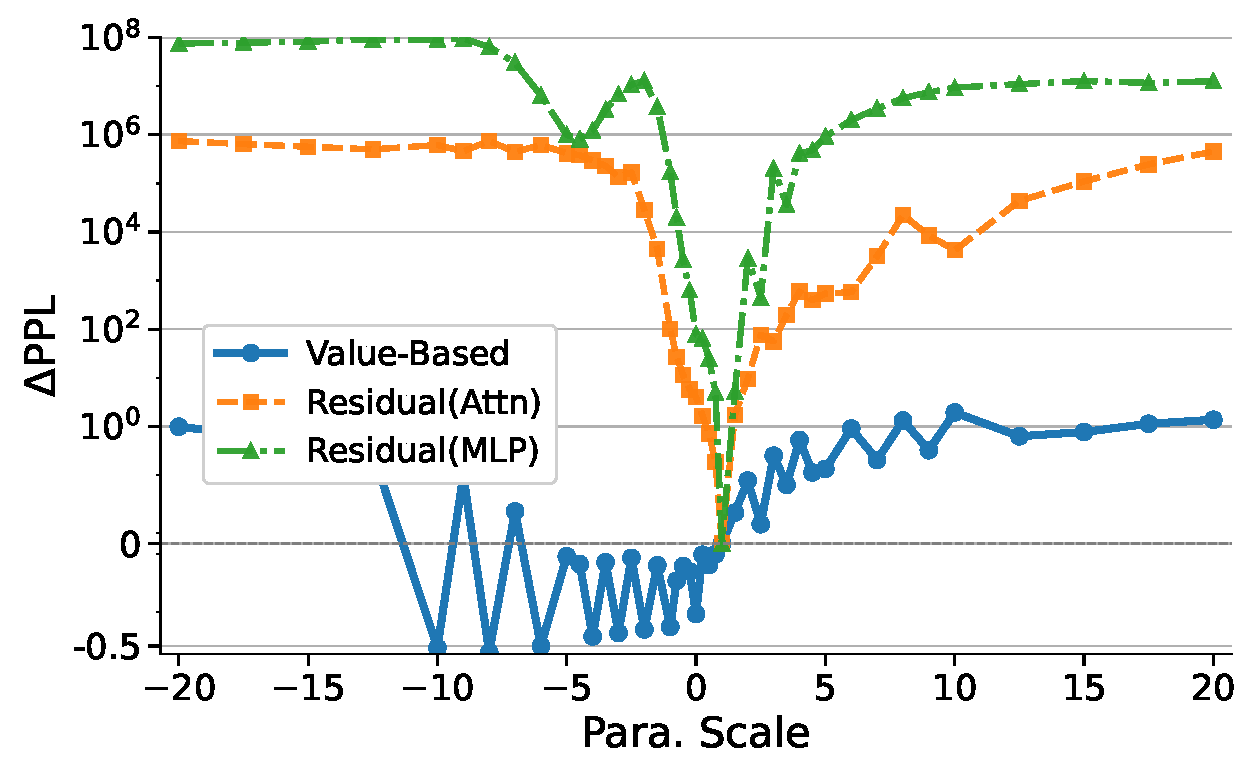
\includegraphics[width=\linewidth]{figs/para_ablation/para_scale_weighted_delta_ppl.pdf}
    \caption{Parallel-component scaling.}
  \end{subfigure}\hfill
  \begin{subfigure}[t]{0.485\linewidth}
    \centering
    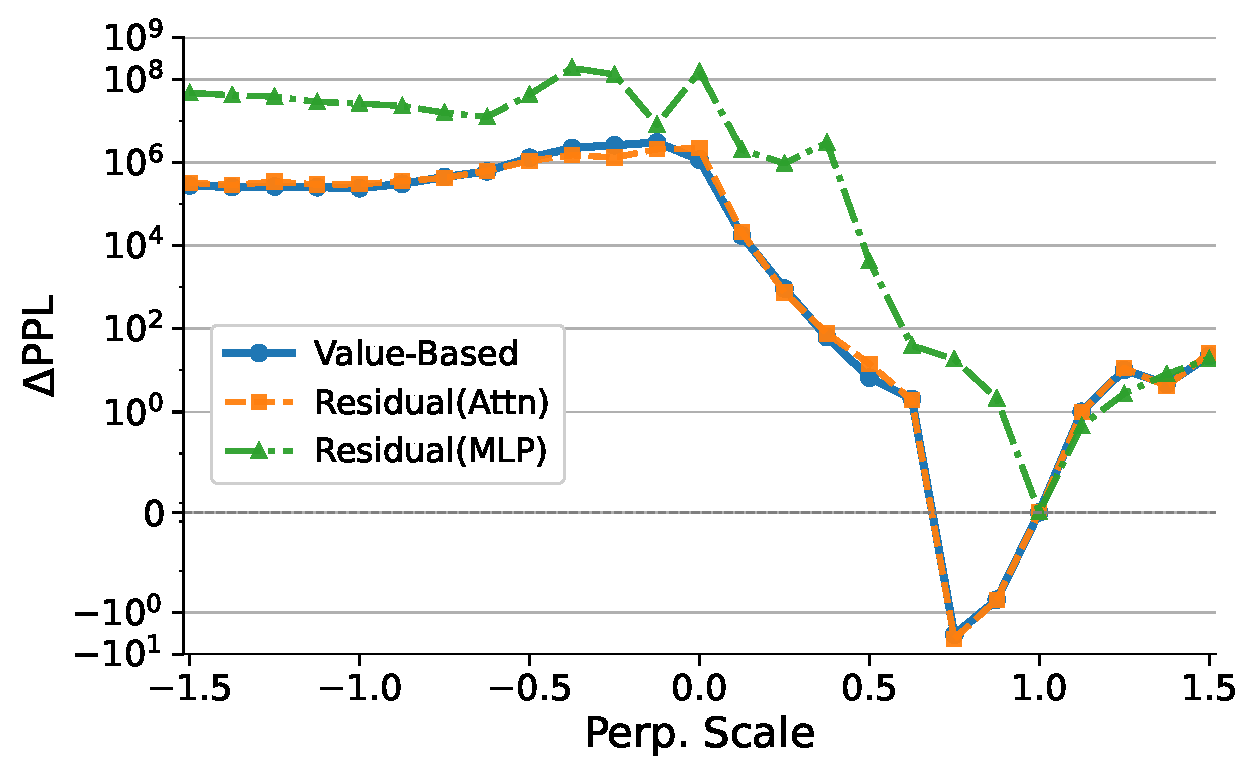
\includegraphics[width=\linewidth]{figs/para_ablation/perp_scale_weighted_delta_ppl.pdf}
    \caption{Perpendicular-component scaling.}
  \end{subfigure}
  \caption{\textbf{Perplexity change under component scaling on Qwen3-4B.}
           We vary \(s_{\parallel}\) (left) or \(s_{\perp}\) (right). Curves
           include value-space manipulation and two residual-space variants.}
  \label{fig:residual-component-editing}
\end{figure}

\paragraph{Component-scaling interpretation.}
Figure~\ref{fig:residual-component-editing} shows that parallel edits are less
disruptive than perpendicular edits on Qwen3-4B over the tested range. Within
this comparison, value-space manipulation stays closest to baseline, Residual(Attn)
is the more robust residual-space variant, and Residual(MLP) is less stable.
This robustness is a property of the value-aggregation coordinate system, not
of every possible parallel direction. The small change in performance over a
wide range of \(s_{\parallel}\) suggests that value-space parallel scaling can
be modified without immediately disrupting the main token-mixing geometry.

Residual(Attn) is less stable because its reference direction is defined only
after \(W_O\) and residual addition, where earlier residual-stream information
has already been mixed in. When translated back to value space, the resulting
diagonal coefficients do not implement a uniform self-value-parallel scaling
across tokens. Appendix~\ref{app:method} gives the corresponding diagonal
derivation. Thus, over the tested range, value-space manipulation stays closest to
baseline, Residual(Attn) is weaker but still comparatively robust, and
Residual(MLP) is fragile. The key question is therefore which coordinate
system makes a parallel edit function-preserving.

\subsection{Value-Space vs.\ Residual-Space Editing}
\label{sec:value-vs-residual-exp}

The preceding results suggest that some parallel components can be modified
with limited behavioral change, but the manipulation space remains important. In
particular, manipulating the self-value-parallel direction need not behave like
a residual-space parallel edit or a hard diagonal mask. The closed-form
analysis in Section~\ref{sec:closed-form-control} shows that these edits act
through different mechanisms, so we compare their zero-shot behavior and the
attention patterns they induce.

\begin{table}[t]
  \caption{\textbf{Zero-shot performance under attention-side edits on Qwen3.}
  We compare baseline, attention-side parallel removal (Attn Para-Rem.), hard
  diagonal removal (Diag. Rem.), and value-space parallel removal
  (V-Para Rem.) on a dense model and an MoE model.}
  \label{tab:general-zeroshot}
  \centering
  \scriptsize
  \setlength{\tabcolsep}{2.6pt}
  \resizebox{\linewidth}{!}{%
  \begin{tabular}{lrrrrrrrr}
    \toprule
    \multirow{2}{*}{Task} & \multicolumn{4}{c}{Qwen3-1.7B} & \multicolumn{4}{c}{Qwen3-30B-A3B} \\
    \cmidrule(lr){2-5}\cmidrule(lr){6-9}
      & Baseline & Attn Para-Rem. & Diag. Rem. & V-Para Rem. & Baseline & Attn Para-Rem. & Diag. Rem. & V-Para Rem. \\
    \midrule
    OpenBookQA & 37.2 & 37.2 & 26.0 & 36.4 & 45.4 & 43.0 & 31.0 & 45.2 \\
    PIQA & 72.1 & 72.0 & 49.4 & 72.1 & 80.2 & 78.8 & 55.9 & 80.8 \\
    RTE & 70.0 & 66.1 & 54.5 & 70.8 & 82.0 & 79.1 & 50.9 & 82.7 \\
    Winogrande & 60.7 & 55.8 & 51.2 & 59.8 & 72.3 & 66.6 & 50.0 & 72.2 \\
    BoolQ & 77.8 & 71.2 & 39.5 & 77.6 & 88.7 & 88.0 & 38.2 & 88.6 \\
    ARC-Challenge & 53.2 & 50.2 & 27.1 & 53.1 & 70.0 & 64.9 & 26.6 & 69.9 \\
    HellaSwag & 60.4 & 58.9 & 26.2 & 60.4 & 77.8 & 73.6 & 33.7 & 77.8 \\
    MMLU & 35.0 & 23.0 & 22.0 & 35.0 & 67.0 & 50.0 & 13.0 & 67.0 \\
    GSM8K & 68.0 & 0.2 & 0.0 & 67.7 & 89.8 & 39.9 & 0.0 & 89.8 \\
    HumanEval & 38.4 & 25.0 & 0.0 & 42.1 & 32.3 & 14.6 & 0.0 & 31.7 \\
    NQ-Open & 9.7 & 7.2 & 0.0 & 9.7 & 25.1 & 16.4 & 0.3 & 25.2 \\
    \midrule
    Avg & 53.0 & 42.4 & 26.9 & 53.2 & 66.4 & 55.9 & 27.2 & 66.4 \\
    \bottomrule
  \end{tabular}}
\end{table}

\paragraph{General zero-shot comparison.}
Table~\ref{tab:general-zeroshot} compares attention-side edits on dense
Qwen3-1.7B and MoE Qwen3-30B-A3B. V-Para Rem. stays close to baseline on most
tasks and gives the strongest edited average. In contrast, Attn Para-Rem. and
hard diagonal removal produce large drops, especially on MMLU, GSM8K, and
HumanEval. This pattern matches the scaling sweep: self-value-parallel
components can be removed with little loss only when the edit follows the
self-value direction.

\paragraph{Long-context zero-shot comparison.}
\begin{wraptable}[8]{r}{0.48\linewidth}
  % \vspace{0.15em}
  \centering
  \caption{\textbf{Long-context RULER performance.}
  Average task-family scores for Llama-3.2-3B.}
  \label{tab:longcontext-ruler}
  \scriptsize
  \setlength{\tabcolsep}{4.2pt}
  \renewcommand{\arraystretch}{0.86}
  \begin{tabular}{lrrrrrr}
    \toprule
    Method & 4k & 8k & 16k & 32k & 64k & 128k \\
    \midrule
    Baseline & 77.2 & 65.6 & 65.1 & 63.8 & 58.8 & 54.8 \\
    Attn Para-Rem. & 52.6 & 48.5 & 48.9 & 48.4 & 45.2 & 39.7 \\
    MLP Para-Rem. & 37.9 & 31.0 & 27.6 & 23.6 & 17.9 & 14.2 \\
    Both Para-Rem. & 56.9 & 47.6 & 41.6 & 34.4 & 24.9 & 20.7 \\
    V-Para Rem. & 76.2 & 65.3 & 65.2 & 63.8 & 59.2 & 54.9 \\
    \bottomrule
  \end{tabular}
  \vspace{-0.8em}
\end{wraptable}
Table~\ref{tab:longcontext-ruler} extends the comparison to long-context
RULER on Llama-3.2-3B. V-Para Rem. tracks the baseline from 4k through 128k,
whereas residual-space branch parallel removal degrades performance across
the range. The ordering from standard zero-shot tasks therefore also appears
in the long-context setting.

\paragraph{Attention diagonal and parallel geometry.}
\label{sec:diagonal-validation}
Value-space parallel removal can be written as an effective diagonal edit, but
it is not equivalent to masking the diagonal entry. The removed-case row in
Table~\ref{tab:effective-diagonal-derivation} shows the key distinction:
value-based removal rewrites the diagonal coefficient using value-space
similarities \(\mathbf{v}_s^\top\mathbf{v}_t/\|\mathbf{v}_t\|^2\), whereas the
residual-space analogue uses post-\(W_O\) similarities against the residual
reference direction. Hard diagonal removal instead sets
\(\widetilde A_{tt}=0\) and renormalizes attention over non-self tokens. The
results in Table~\ref{tab:general-zeroshot} therefore show that parallel
redundancy is direction-sensitive: parallel removal stays close to baseline
only when the edit is aligned with the self-value-parallel direction.

\paragraph{Attention-map view.}
\label{sec:attn-map-analysis}
\begin{wrapfigure}{r}{0.49\linewidth}
  \centering
  \vspace{-1.2em}
  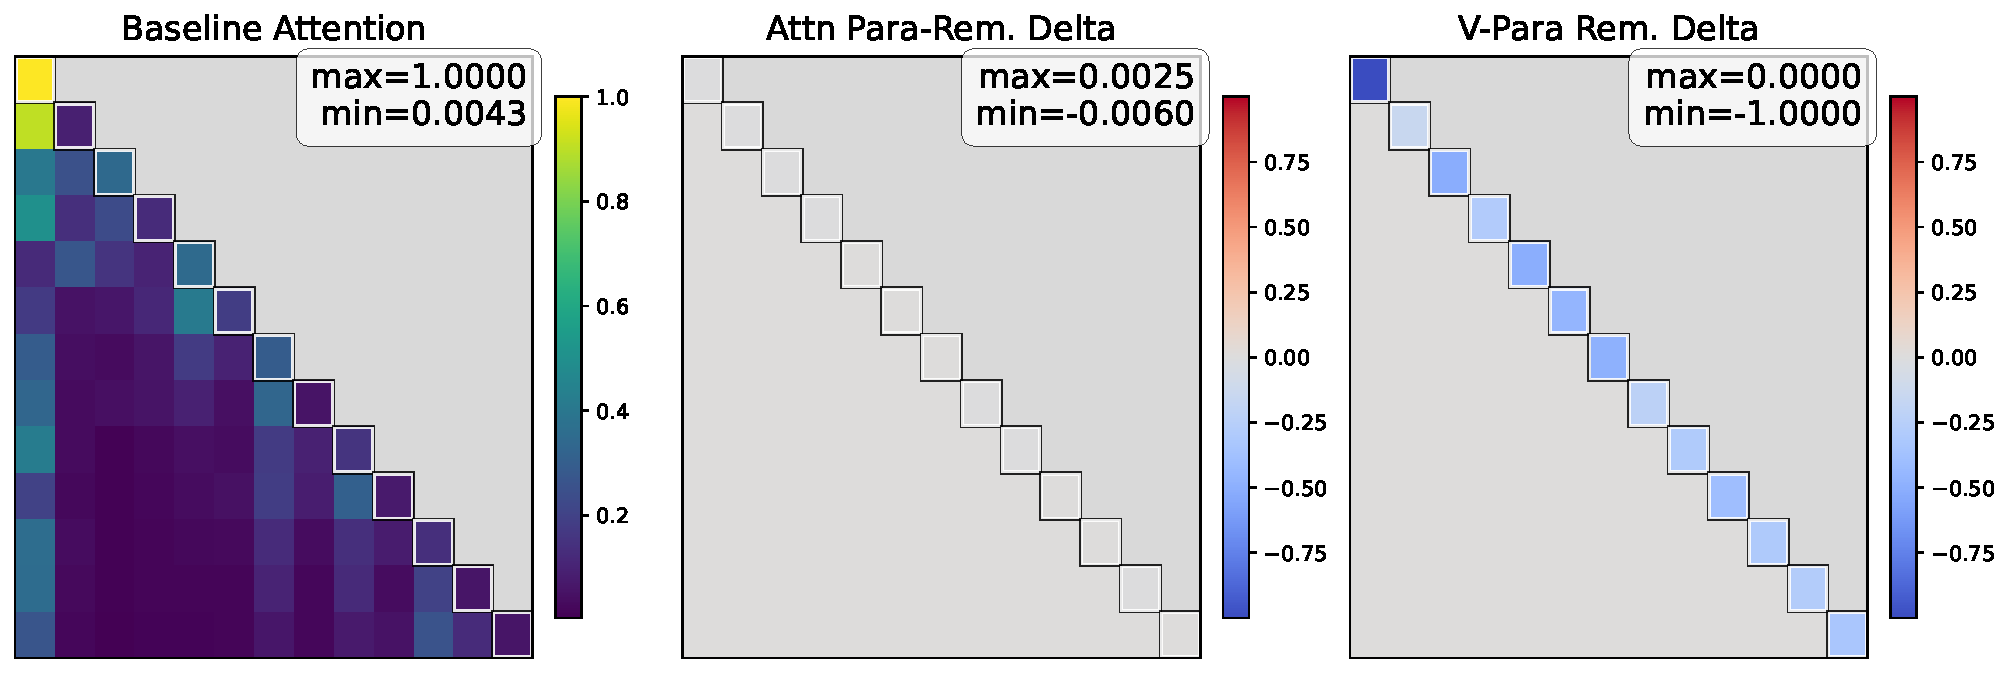
\includegraphics[width=\linewidth]{figs/attn_matrix/outputs/qwen3-4b/layer19/h6_three_map_compare.pdf}
  \caption{\textbf{Diagonal-edit attention maps on Qwen3-4B.}
  We compare a layer-19 head under baseline, hard diagonal removal, and
  value-space parallel removal.}
  \label{fig:attn-maps}
  \vspace{-0.6em}
\end{wrapfigure}
Figure~\ref{fig:attn-maps} illustrates how the diagonal edits change token
mixing on Qwen3-4B. Hard diagonal masking removes the self entry and
renormalizes over non-self tokens, which can concentrate probability mass on a
small set of off-diagonal positions. In contrast, V-Para Rem. changes the
self-value-parallel contribution without imposing this hard row-level
redistribution. This qualitative view matches the benchmark results: the edit
space matters more than the diagonal entry alone.

% ------------------------------------------------------------------
\subsection{Compression-Induced Error Geometry}
\label{sec:compression-error-geometry}

\begin{wrapfigure}{r}{0.5\linewidth}
  \centering
  \vspace{-0.8em}
  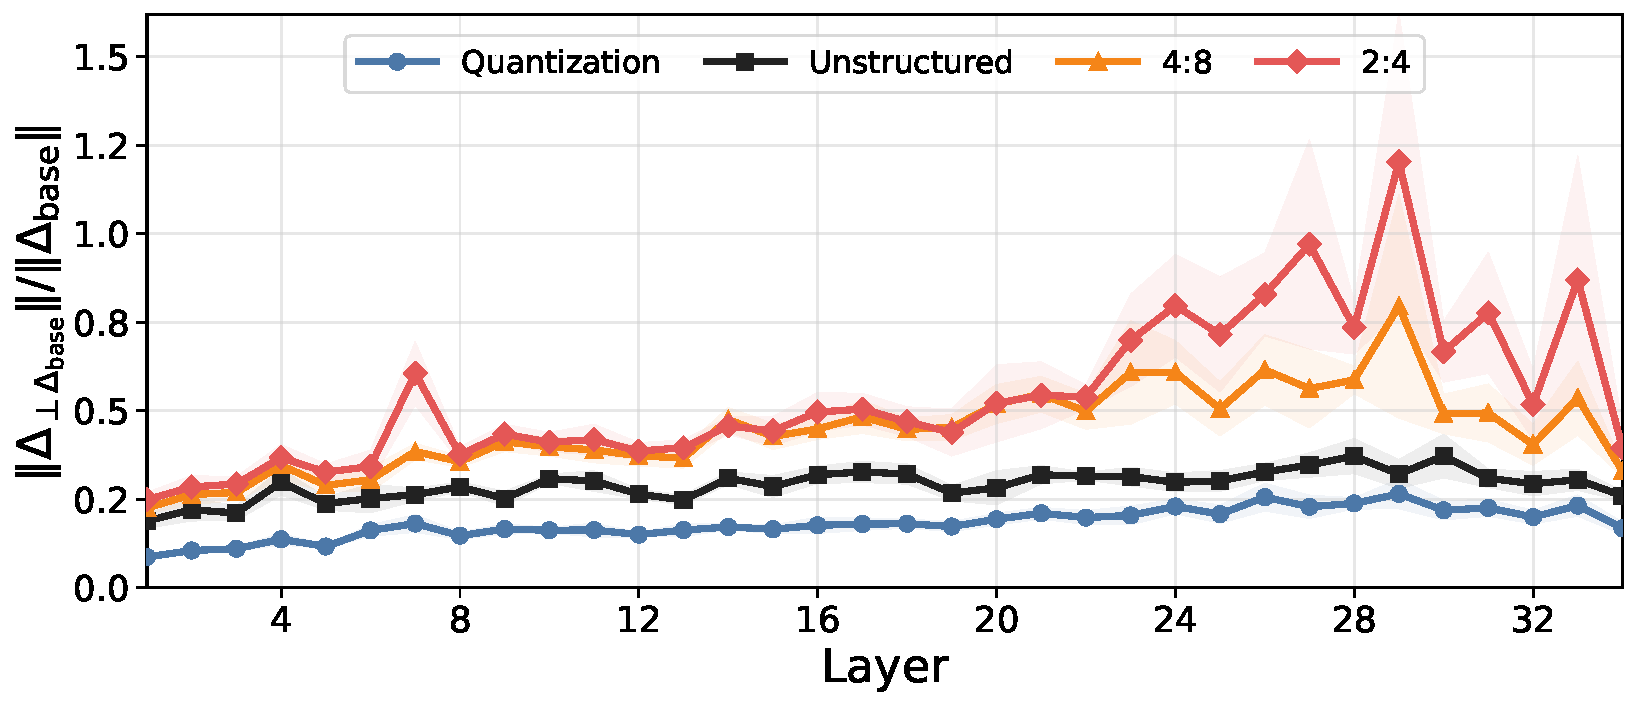
\includegraphics[width=\linewidth]{figs/comp_analysis/local_flip_compare-attn_out-perp_over_base_update.pdf}
  \caption{\textbf{Residual-space error geometry under attention compression.}
  We measure the perpendicular component of attention-output compression error,
  normalized by the baseline update.}
  \label{fig:local-flip-attn}
  \vspace{-1.5em}
\end{wrapfigure}

Model compression introduces approximation error into residual updates, making
it a natural setting for testing whether residual-error geometry predicts
downstream degradation. Figure~\ref{fig:local-flip-attn} reports the
perpendicular component of the attention-output compression error, normalized
by the baseline update. Appendix~\ref{app:compression} provides the branch-wise
and parallel-error views.

Figure~\ref{fig:local-flip-attn} shows that attention-compression settings
with smaller perpendicular error remain better aligned with the baseline
residual update. Parallel error is less discriminative than perpendicular
error, matching the component-scaling experiments above. This suggests a
label-free diagnostic for compression: candidate compressed models can be
screened by how much perpendicular residual error they introduce.

\subsection{Pretraining Optimization}
\label{sec:pretraining}

The inference and compression experiments indicate that parallel and
perpendicular components play different functional roles. This motivates a
training-side test: if the self-value-parallel direction can be modified with
limited inference-time degradation, then suppressing that component during
training may change the optimization trajectory.
We therefore focus on parallel-removal training runs in the main text and
use Appendix~\ref{app:training-configs} for the training configurations and
the gated scale diagnostic.

\begin{figure}[t]
  \centering
  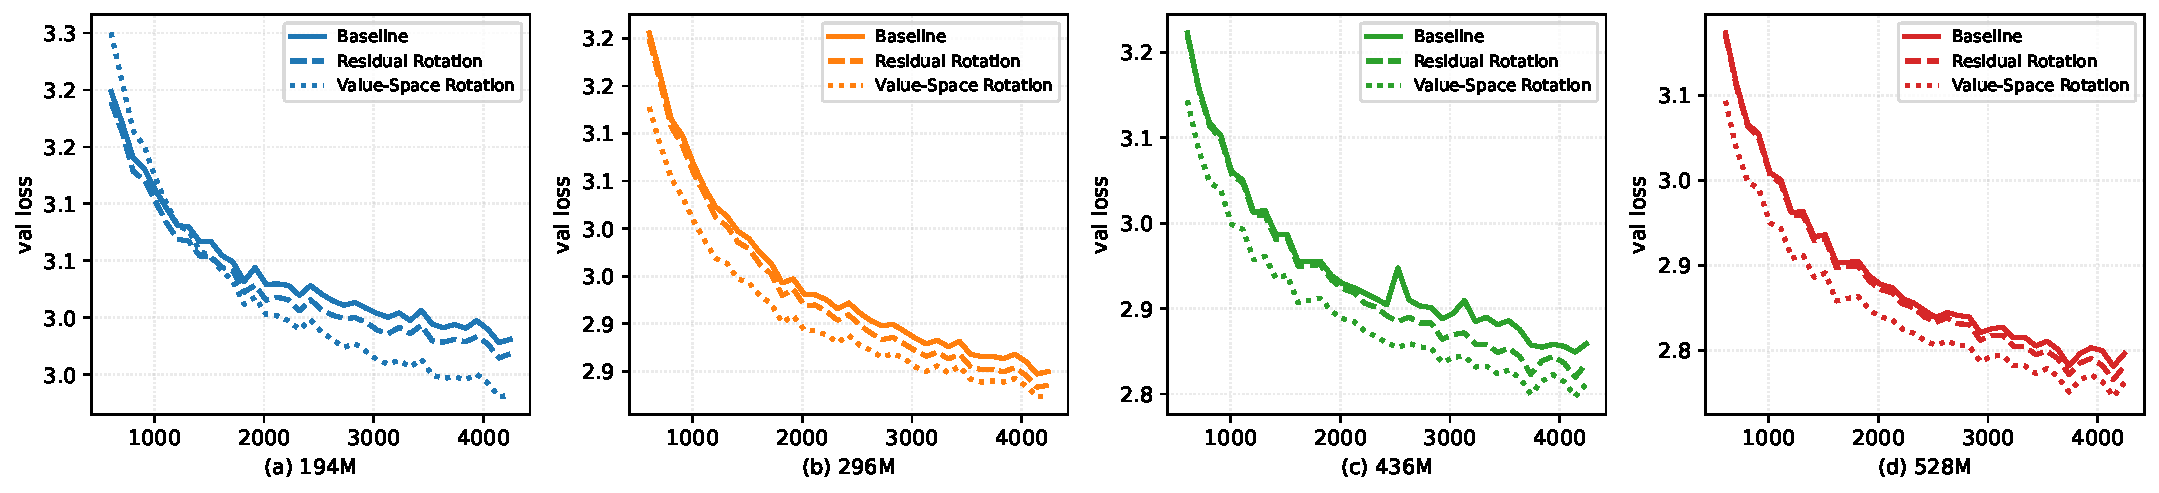
\includegraphics[width=0.98\linewidth]{figs/loss_curves/pretraining_loss_by_size.pdf}
  \caption{\textbf{Small-model pretraining under parallel removal.}
  We compare baseline training with attention-side parallel-removal runs
  across model sizes.}
  \label{fig:pretraining}
\end{figure}

Figure~\ref{fig:pretraining} shows that attention-side parallel removal changes
the optimization trajectory. The separation from baseline appears early in
training and remains visible across model sizes, indicating that the
intervention affects how the model allocates learning rather than only the
final checkpoint.

\begin{table*}[t]
  \caption{\textbf{Post-training benchmark performance across model scale.}
  We compare baseline, attention-side parallel removal, and value-space
  parallel removal on larger pretraining runs.}
  \label{tab:pretraining-summary}
  \centering
  \scriptsize
  \setlength{\tabcolsep}{4pt}
  \resizebox{\textwidth}{!}{%
  \begin{tabular}{llrrrrrrrr}
    \toprule
    Model & Setting & ARC-E & BoolQ & HSwag & OBQA & PIQA & WinoGr & Avg & $\Delta$Avg \\
    \midrule
    \multirow{3}{*}{1.4B}
      & Baseline & 56.0 & \textbf{65.1} & 60.5 & 34.7 & 75.8 & 58.7 & 58.5 & -- \\
      & Attn Para-Rem. & 57.1 & 63.9 & 61.3 & 35.3 & 76.0 & 59.1 & 58.8 & +0.3 \\
      & V-Para Rem. & \textbf{58.3} & 62.8 & \textbf{62.1} & \textbf{35.9} & \textbf{76.3} & \textbf{59.8} & \textbf{59.2} & \textbf{+0.7} \\
    \midrule
    \multirow{3}{*}{2.7B}
      & Baseline & 58.4 & 61.2 & 66.0 & 37.1 & 76.5 & 61.8 & 60.2 & -- \\
      & Attn Para-Rem. & 59.3 & 62.8 & 66.7 & 37.7 & 77.0 & 62.1 & 60.9 & +0.8 \\
      & V-Para Rem. & \textbf{60.4} & \textbf{64.4} & \textbf{67.1} & \textbf{38.2} & \textbf{77.6} & \textbf{62.6} & \textbf{61.7} & \textbf{+1.6} \\
    \bottomrule
  \end{tabular}}
\end{table*}

Table~\ref{tab:pretraining-summary} reports downstream evaluation for the
larger pretraining runs. Attn Para-Rem. improves the average score over
baseline, and V-Para Rem. gives the strongest average improvement at both
scales. Together with the loss curves, these results are consistent with the
view that suppressing self-value-parallel components changes the optimization
trajectory. The gated scale diagnostic in Appendix~\ref{app:training-configs}
serves as supporting evidence rather than the main training result.
